\chapter{Помехоустойчивое кодирование}

\section{Введение}

Современные системы связи сталкиваются с проблемой ошибок передачи данных, вызванных шумами и помехами в каналах связи. Для обеспечения надежности передачи используется метод помехоустойчивого кодирования, который позволяет обнаруживать и исправлять ошибки.

Одним из таких методов является \textbf{сверточное кодирование}, которое добавляет избыточность в передаваемое сообщение, повышая его устойчивость к ошибкам. Для декодирования закодированных данных применяется \textbf{алгоритм Витерби}, позволяющий эффективно восстанавливать исходное сообщение даже при наличии искажений.

\section{Сверточное кодирование}

Сверточное кодирование относится к классу линейных кодов, где выходные данные зависят не только от текущего входного бита, но и от предыдущих битов. Данный метод используется в цифровых системах связи и хранения данных благодаря своей эффективности.

\subsection{Принцип работы}

Процесс кодирования осуществляется с использованием \textbf{кодирующего регистра сдвига} и \textbf{кодирующих полиномов}. Для данной работы используется схема кодирования с параметрами:

- \textbf{Скорость кодирования}: $1/2$ (на один входной бит генерируется два выходных);
- \textbf{Кодирующие полиномы}: $G_1 = 171_8$, $G_2 = 133_8$;
- \textbf{Очередность выхода}: поочередное поступление битов с выходов $X, Y, X, Y, ...$.

Входное сообщение последовательно проходит через сдвиговый регистр, а выходные биты формируются путем побитового сложения по модулю 2 (операция XOR) в соответствии с кодирующими полиномами.

\subsection{Структура кодера}

На рисунке \ref{fig:encoder} представлена схема сверточного кодера с двумя выходными потоками:

\begin{figure}[h]
    \centering
    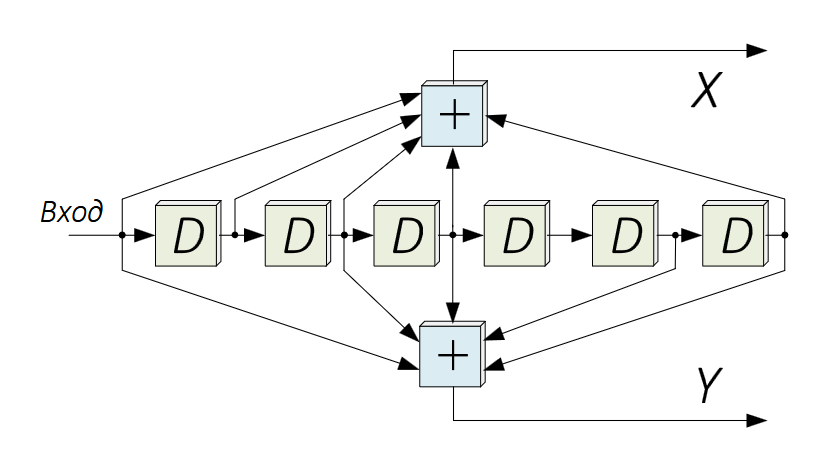
\includegraphics[width=0.7\textwidth]{encoder.png}
    \caption{Схема сверточного кодера}
    \label{fig:encoder}
\end{figure}

Входные биты проходят через регистры сдвига, формируя новые выходные биты по заданным полиномам. В результате длина закодированного сообщения в два раза превышает длину исходного.

\section{Декодирование методом Витерби}

Для восстановления исходного сообщения применяется \textbf{алгоритм Витерби}, который представляет собой метод поиска оптимального пути в решетчатом графе возможных состояний кодера.

\subsection{Основная идея алгоритма}

1. Строится \textbf{решетчатая диаграмма}, отображающая все возможные переходы состояний кодера.
2. На каждом шаге сравниваются принятые биты с ожидаемыми, вычисляется мера расхождения (метрика Хэмминга).
3. Выбираются пути с минимальной метрикой, исключая наименее вероятные траектории.
4. В конце пути восстанавливается наиболее вероятная последовательность входных битов.

\subsection{Коррекция ошибок}

Метод Витерби позволяет исправлять ошибки, возникшие в канале передачи. Чем длиннее передаваемая последовательность, тем выше вероятность корректного восстановления данных.

\section{Выводы}

В данной главе рассмотрены методы сверточного кодирования и декодирования с использованием алгоритма Витерби. Основные выводы:

- Сверточное кодирование повышает устойчивость данных к шумам, добавляя избыточность.
- Алгоритм Витерби позволяет эффективно декодировать сообщение, минимизируя вероятность ошибок.
- Данный метод широко применяется в цифровой связи, включая спутниковые и мобильные системы.

Использование помехоустойчивого кодирования критически важно для обеспечения надежности передачи информации в условиях реальных каналов связи.

